\label{chapter:coordinatingstorage}


% As a general rule, do not put math, special symbols or citations
% in the abstract
%\begin{abstract}

%A batch processing job in a distributed system has three clear steps, stage-in, execution, and stage-out.  As data sizes have increased, the stage-in  time has also increased.  In order to optimize stage-in time for shared inputs, we propose the CacheD, a caching mechanism for high throughput computing.  Along with caching on worker nodes for rapid transfers, we also introduce a novel transfer method to distribute shared caches to multiple worker nodes utilizing BitTorrent.  We show that our caching method significantly improves workflow completion times by minimizing stage-in time while being non-intrusive to the computational resources, allowing for opportunistic resources to utilize this caching method.


%\end{abstract}

This chapter is a combination of the following publication and additional work that is being prepared for publication.

\bibentry{weitzel2015pdpta}




\section{Introduction}

Large input datasets are becoming common in scientific computing.  Unfortunately for campus researchers, the staging time of the datasets to computational resources has not kept pace with the increase in dataset sizes.  The typical large dataset workflow may consist of thousands of individual jobs, each sharing input files.  

The campus resources made available to researchers are shared; therefore, the researchers have the limitation of not having access to install programs on the clusters.  Previous work \cite{weitzel2014accessing} built an overlay on top of campus resources to create a virtual, on-demand pool of resources for task execution.  We expand the capabilities of this virtual pool to include data caching and novel transfer methods to enable big data processing.

%Each node in the virtual pool will run multiple jobs, by default, all batch systems will transfer the large input file for each job.  Our goal is to minimize the number of times the input data is transferred from the submit host to the execution target.  Therefore a framework of local caching and distributed file transfer is proposed to address these situations.

An excellent example of a big data workflow is that of the bioinformatics application: BLAST \cite{altschul1997gapped}.  Each BLAST query requires an entire reference database, which can range in size from a few kilobytes to many gigabytes.  The workflow to run a BLAST query requires a large stage-in time in order to make the reference database available.  Additionally, the databases are frequently updated with new entries.

Users in the past have copied the database using various methods.  The na\"{i}ve method includes copying the database for each job.  Storing the database on a shared filesystem has the same effect as copying the database for each job, since the database must be transferred to the execution node for each job.  We propose caching the database on the node for subsequent executions.

We find that the BLAST workflow described above is common among large data researchers.   

Bosco \cite{weitzel2014accessing} is a remote submission tool that can create overlay virtual pools designed for campus resources.  In previous work, Bosco allowed campus researchers to submit high throughput jobs to high performance clusters.  We extend Bosco to include data caching and novel data transfer methods. 

We limit our design and analysis to a campus cluster computing environment.  Our solution is unique in that it is designed to run opportunistically on the campus computing resources.  Additionally, they do not require administrator intervention in order to create a virtual, on-demand pool of resources.


\section{Background and Related Work}

% Background on caching

Data caching on distributed systems has been used many times and at many levels.  Caching can be done on the storage systems and on the execution hosts, as well as well as in within the infrastructure separating the two.

Some distributed filesystems use local caches on the worker nodes.  GPFS \cite{schmuck2002gpfs} has a read-only cache on each worker node that can cache frequently accessed files.  It is designed for a fast, shared filesystem and is recommended when file access latency is a concern.  It is not recommended for large files since internal bandwidth to the local disk is assumed to be less than the bandwidth available to the GPFS shared filesystem.  GPFS file transfers are typically done over high speed interconnects which can provide high bandwidth for large files.  These interconnects are not typically available to a user's jobs for transferring data from a remote source.

% pcache?

% HTTP caching
HTTP caching is used throughout the web to decrease latency for page loads and to distribute requests among servers.  In high throughput computing, a forward proxy is commonly used to cache frequent requests to external servers.  The forward proxy caches files requested through it, and will respond to subsequent requests for the same file by reading it from memory or its own disk cache.

The HTTP forward proxy caching does have limitations.  The HTTP protocol was designed and is used primarily for websites.  Websites have very different requirements from high throughput computing.  The data sizes are much smaller.  Software designed as forward proxies, such as Squid \cite{squidcacheurl}, are optimized for web HTTP traffic, and therefore do not handle large data file sizes optimally.  Further, the Open Science Grid (OSG) \cite{pordes2007open} sites typically only have one or possibly a few squid caches available to user jobs.  They are not designed to scale to large transfers for hundreds of jobs, our target use case.

% chirp / parrot
Parrot \cite{thain2005parrot} is another application that will cache remote files when using certain protocols.  Parrot uses interposition \cite{thain2001multiple} to capture and interpret IO operations by an unmodified binary application.  The interposition allows Parrot to provide a transparent interface to remote data sources.  Parrot caches some of those sources such as HTTP with GROW-FS, a filesystem using HTTP.  Parrot caches an entire file to the local storage.  Parrot must download directly from the source the first time it is requested, exhausting WAN bandwidth quickly for large files.


% CernVM-FS
CernVM-FS \cite{blomer2011cernvm} provides a filesystem over the HTTP protocol.  It integrates into the worker node system using the FUSE \cite{szeredi2010fuse} interface.  The CernVM-FS local node client caches files on the node, as well as using Squid to cache files at the site.  Again, since it uses the HTTP, it's not designed to cache large files.  Neither the Squid caches nor the web servers optimally transfer large files, nor are they designed for large data sizes.  Further, CernVM-FS requires administrator access in order to install and configure, a privilege that campus users do not have.


% xrootd caching
XrootD \cite{dorigo2005xrootd} is designed for large data access, and it has even been used for WAN data transfers \cite{bauerdick2012using} using a federated data access topology.  There has been some work in creating a caching proxy for the XrootD \cite{bauerdick2014xrootd}.  The caching proxy is designed to cache datasets on filesystems near the execution resources.  The caching proxy requires installation of software and the running of services on the cluster.  Unprivileged campus users will be unable to run or install these services.



% transfer protocols
% HTTP

% Caching in the 
We define local caching as saving the input files on the local machine and making them available to local jobs.  Local caching is different from site caching, which is done in the OSG by Squid caches.  We define site caching as when data files are stored and available to jobs from a closer source than the original.  In most cases on the OSG, the site cache is a node inside the cluster that has both low latency and high bandwidth connections to all of the execution hosts.

%BitTorrent
We use distributed transfer to mean transfers that are not from a single source.  In our case, we will be using BitTorrent \cite{cohen2008BitTorrent}, in which a client may download parts of files from multiple sources.  Additionally, the client may make available to other clients parts of the files that have already been downloaded.

BitTorrent is a transfer protocol that is designed for peer-to-peer transfers of data over a network.  It is optimized to share large datasets between peers. The authors of \cite{wei2005scheduling} and \cite{wei2007towards} discuss scheduling tasks efficiently in peer-to-peer grids and desktop grids.  Their discussion does not take into account the network bottlenecks that are prevalent in campus cluster computing.  

In \cite{briquet2007scheduling}, the authors use scheduling, caching, and BitTorrent in order to optimize the response time for a set of tasks on a peer-to-peer environment.  They build the BitTorrent and caching mechanisms into the middleware which is installed and constantly running on all of the peers.  They do not consider the scenario of opportunistic and limited access to resources.  Their cluster size is statically set, and therefore may not see the variances that users of campus clusters may see.



\section{Implementation}



The HTCondor CacheD is a daemon that runs on both the execution host and the submitter.  For our purposes, a cache is defined as an immutable set of files that has metadata associated with it.  The metadata can include a cache expiration time, as well as ownership and acceptable transfer methods.


\begin{figure}[ht]
\centering
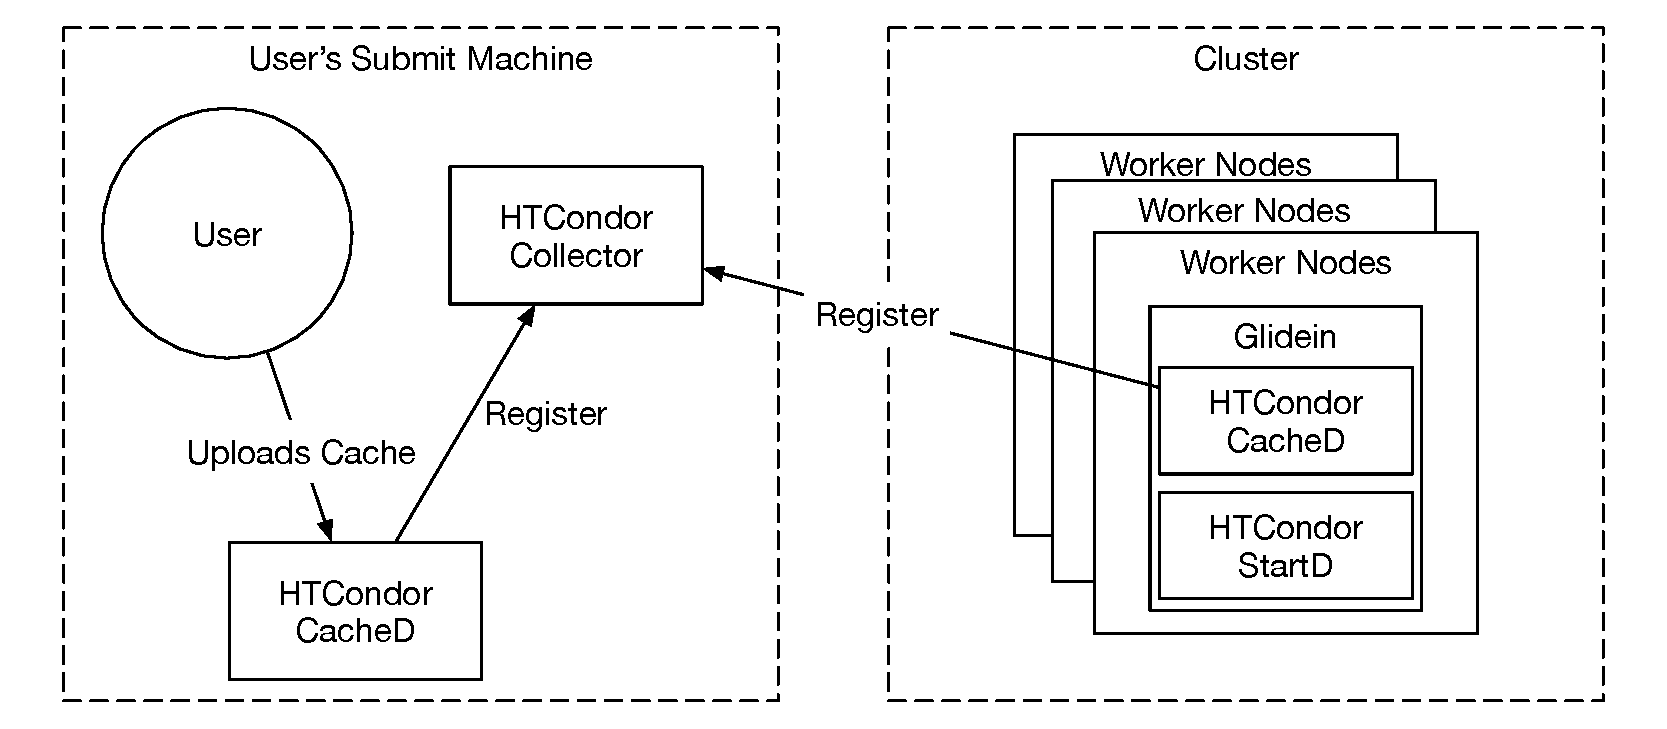
\includegraphics[width=\textwidth]{images/DaemonLayout.pdf}
\caption{Daemon Locations}
\label{fig:daemonlayout}
\end{figure}


The CacheD follows the HTCondor design paradigm of a system of independent agents cooperating.  Each CacheD makes decisions independently of each other.  Coordination is done by CacheD�s communicating and negotiating with each other.

Each caching daemon registers with the HTCondor Collector.  The collector serves as a catalog of available cache daemons that can be used for replication.

% Talk about the transfer plugin
In addition to the CacheD, a transfer plugin is used to perform the cache transfers in the job's sandbox.  The plugin uses an API to communicate with the local CacheD to request local replication requests to the local host.  After the cache is transferred locally, the plugin then downloads the cache to the job's working directory.

Expiration time is is used for simple cache eviction.  A user creates a cache with a specific expiration time.  After a cache has expired, a caching server may delete it to free space for other caches.  The expiration may be requested to be extended by the user 

The CacheD supports multiple different forms of transferring data.  Using HTCondor's file transfer plugin interface, it can support pluggable file transfers.  For this paper, we will only use the BitTorrent and Direct transfer methods.  The BitTorrent method uses the libtorrent library to manage BitTorrent transfers and torrent creation.  The Direct method uses an encrypted and authenticated stream to transfer data from the source to the client.

An important concept of the caching framework is a cache originator.  The original daemon that the user uploaded their input files to is the cache originator.  The cache originator is in charge of distributing replication requests to potential nodes, as well as providing the cached files when requested.

The caching daemons interact with each other during replication requests.  A cache originator sends replication requests to remote caching daemons that match the replication policy that is set by the user.  The remote caching daemon then confirms that the cache data can be hosted on the server.  The remote cache then initiates a file transfer in order to transfer the cached data from the origin to the remote CacheD.

The receiving CacheD can deny a replication request for many reasons, including:
\begin{itemize}
\item The resource does not have the space to accommodate the cache.
\item The resource may not have the necessary bandwidth available in order to transfer the cache files.
\item The resource does not expect to be able to run the user's jobs and has determined that the cached files will not be used.
\end{itemize}

The ability of the receiving CacheD to deny a replication request follows HTCondor's independent agent model.

The policy expression language is modeled after the matchmaking language in the HTCondor system \cite{raman1998matchmaking}.  The caching daemon is matching the cache contents to a set of resources; therefore, it is natural to use HtCondor's same matchmaking language that is used to match jobs to resources.  Once a resource is determined to match the cache's policy expression, the caching daemon will contact the resource's caching daemon in order to initiate a cache replication.  The caching daemon on the remote resource is an independent agent that has the ability to deny a caching replication even after matchmaking is successful.  

Libtorrent is built into the CacheD to provide native BitTorrent functionality.  The CacheD is capable of creating torrents from sets of files in a cache, as well as downloading cache files using the BitTorrent protocol.  Since this is a distributed set of caches, we will not use a static torrent tracker.  Rather, we will use a Distributed Hash Table \cite{dinger2009decentralized} and local peer discovery \cite{legout2007clustering} features of the BitTorrent protocol.  This ensures that there are no single points of failure.



\subsection{Creation and Uploading Caches}
The user begins using the caching system by uploading a cache to their own CacheD, which then becomes the cache originator.  This is very similar to a user submitting a job to their own HTCondor SchedD.  Using the cache's metadata, the CacheD decides whether to accept or reject the cache.  If the CacheD accepts the cache, it stores the metadata into resilient storage.  The user then proceeds to upload the cache files to the CacheD.

The CacheD stores the cache files into it�s own storage area.  Once uploaded, the CacheD takes action to prepare the cache to be downloaded by clients.  This includes creating a BitTorrent torrent for the cached files.  

Numerous protections are used in order to ensure proper usage of the CacheD.  The upload size is enforced to the size advertised in the metadata.  The client cannot upload more data to the CacheD than was originally agreed upon during cache creation.  Further, the ownership of the cache is stored in the metadata, and is acquired by authenticating with the client upon cache creation.  Only the owner may upload and download files from the cache directly.

A client may mark a cache as only allowing certain replication methods.  This can be useful if a user wishes to keep data private. BitTorrent doesn't offer the authorization framework to ensure privacy of caches. Users may mark the cache as only allowing DIRECT replications, which are encrypted and authenticated.

\subsection{Downloading Caches}
When a job starts, the CacheD begins to download the cache file.  The cache is identified by a unique string that includes the cache's name and the cache's originator host.  The flow of replication requests is illustrated in Figure \ref{fig:replicationflow}.  The replication requests originate from the file transfer plugin, which sends the replication request to the node local CacheD.  The node local CacheD then sends the replication to its parent or the origin cache.  The propagation of replication requests are modeled after well-known caching mechanisms such as DNS.

\begin{figure}[ht]
\centering
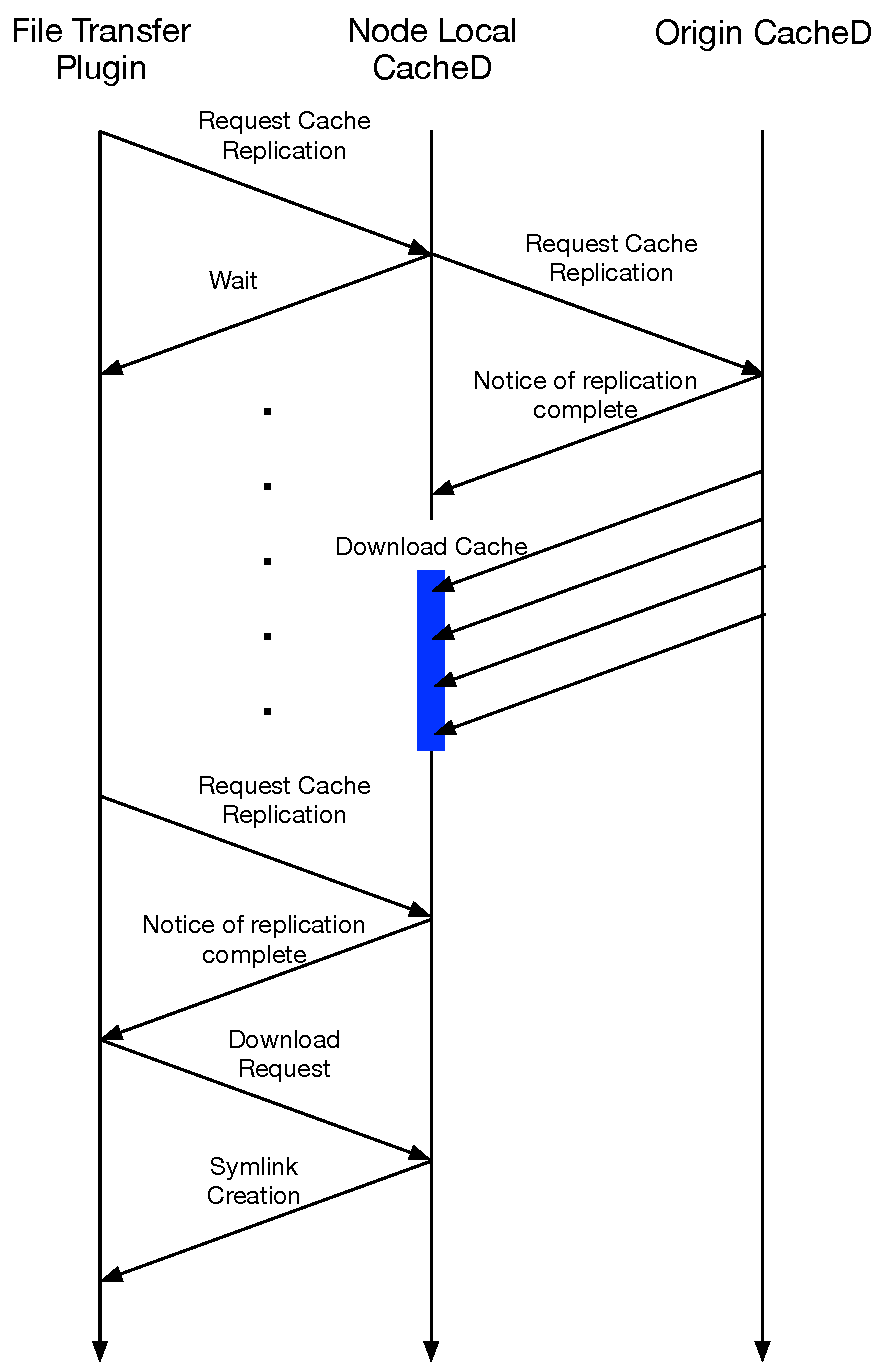
\includegraphics[width=0.5\textwidth]{images/CacheDownloadFlow.pdf}
\caption{Flow of Replication Requests}
\label{fig:replicationflow}
\end{figure}

\begin{enumerate}
\item The plugin contacts the node local CacheD daemon on the worker node.  It requests that the cache is replicated locally in order to perform a local transfer.
\item The node local CacheD responds to the file transfer plugin with a ``wait'' signal.  The file transfer plugin polls the node local CacheD periodically to check on the replication request.
\item The local CacheD daemon propagates the cache replication request to its parent, if it exists.  If the CacheD does not have a parent it contacts the cache originator in order to initiate a cache replication.
\item If the cache is detected to be transferable with BitTorrent, the download begins immediately after receiving the cache's metadata from the parent or origin.
\item Once the cache is replicated locally, the plugin downloads the files from the local CacheD.
\end{enumerate}






Each download is negotiated for the appropriate transfer method between the parent and the client.  Between parent and client CacheD's, the cache's individual replication preferences are honored.  Between a CacheD and the transfer plugin, an additional protocol is offered: symbolic link (symlink).

If the transfer plugin successfully authenticates with a local CacheD, transfer methods are negotiated.  If supported, the symlink method may be chosen.  The symlink transfer method allows near instant transfer of the cache from the CacheD to the plugin.  A symlink is created by the CacheD in the job's working directory pointing to the cache directory.  This symlink method eliminates transferring the cache to each job.

\begin{figure}[ht]
\centering
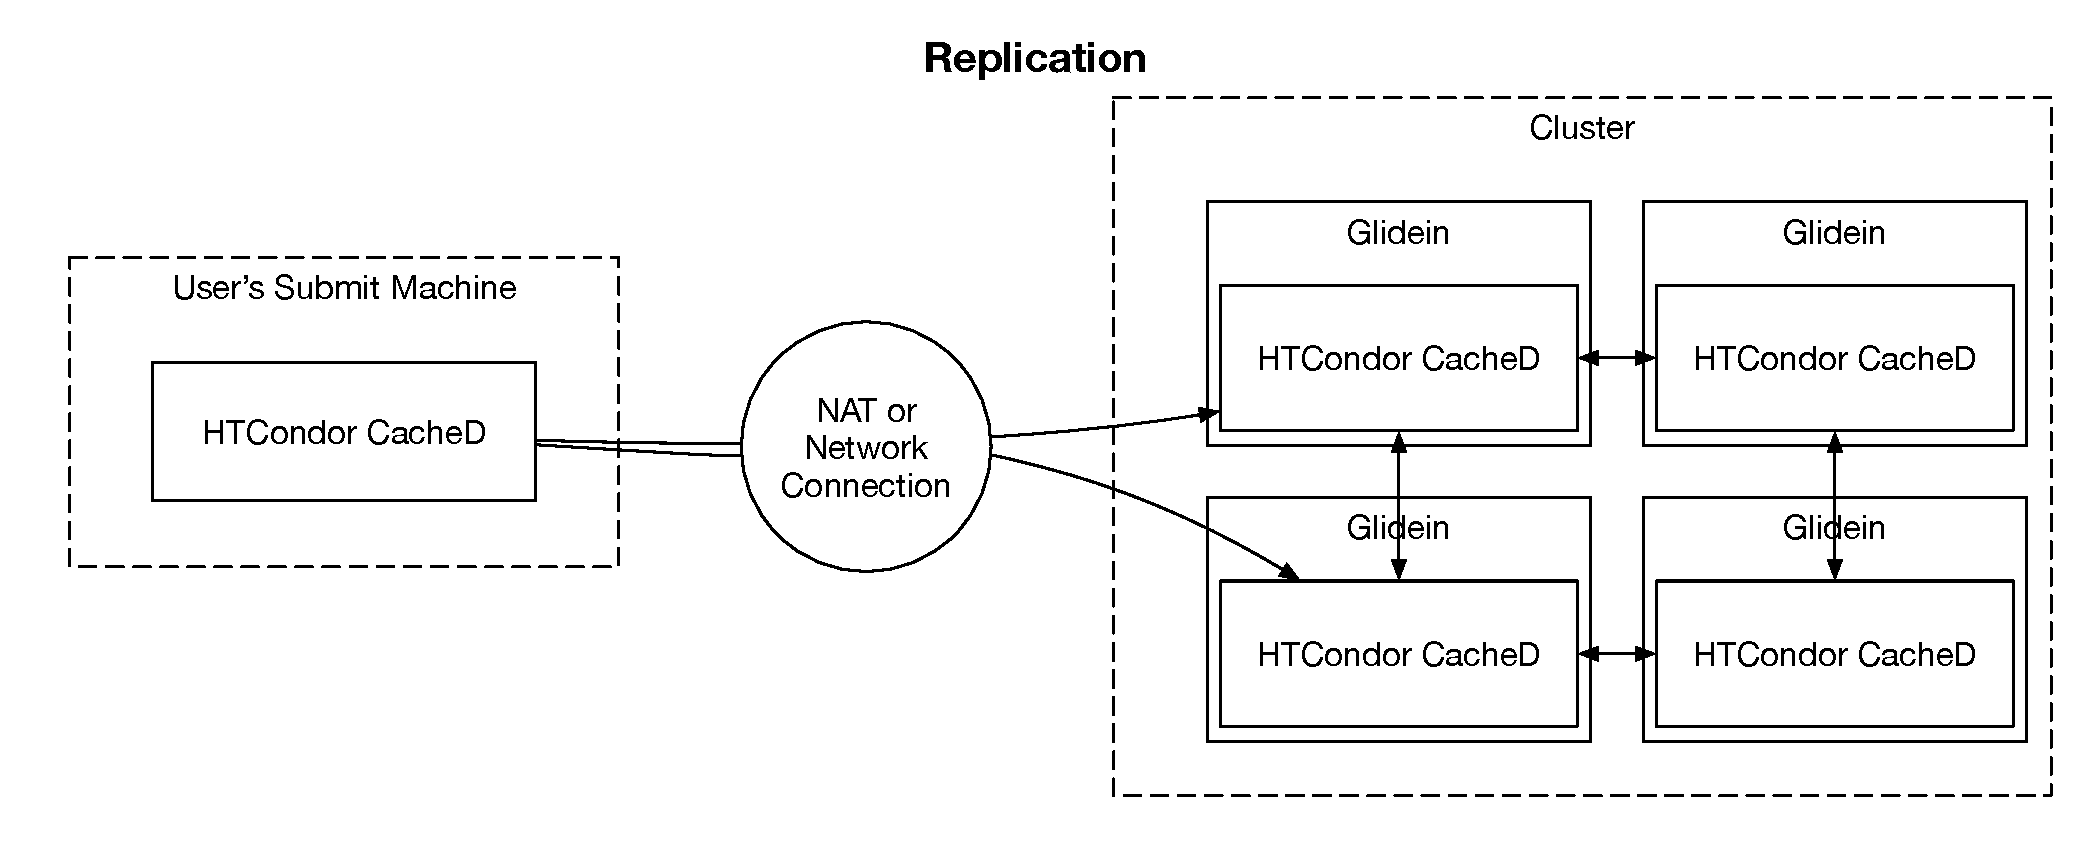
\includegraphics[width=\textwidth]{images/ReplicationBottleneck.pdf}
\caption{Cache Replication Showing Bottleneck}
\label{fig:cachebottleneck}
\end{figure}

In Figure \ref{fig:cachebottleneck}, you can see a traditional configuration of a cluster.  The configuration shows that there is a Network Address Translation bottleneck or a network bottleneck between the submit machine and the execution nodes.  The bottleneck limits the bandwidth between the submit machine and the execution nodes.

% Discuss the possiblity of jobs modifying the cache?


\subsection{Parenting of CacheDs}
During testing of the CacheD, it was apparent that BitTorrent increases the IO queue on the host server significantly, degrading the IO performance for all jobs on the server.  This increased IO queue leads to competition between BitTorrent-enabled CacheD's on the same host.  In order to address the increased IO queue, each CacheD will designate a single daemon on the host that downloads the files through BitTorrent.  All other CacheD�s will then download the cache from the parent using Direct file transfer mechanisms.  

\section{Results}

\subsection{Experimental Design}
To evaluate our solution, we will run a BLAST benchmark from UC Davis \cite{blastbenchmark}.  We chose a BLAST benchmark due to many factors.  BLAST is used frequently on campuses, but used infrequently on clusters due to the size of the database. BLAST has very large databases that are required by each job.  This makes it difficult to use on distributed resources since each job requires significant data.
BLAST databases are frequently updated, making them poor candidates for static caching, but good candidates for short-term caching, for which our CacheD specializes.

The BLAST database distributed with the benchmark is a subset of the Nucleotide NR database.  In our tests, we will use a larger subset of the NR database in order to demonstrate the efficiency of our solution.

For researchers, the time to results is likely the most important metric.  The stage-in time of data can be a large component of the entire workflow time.  We will measure the time for stage-ins as well as the average stage-in time.

We designed two experiments that represent our experience on campus infrastructure.  In the first experiment, we will allow 100 simultaneous jobs to start at the same time and measure the average download time versus the number of distinct nodes.  This experiment also includes the download time for child caches.  We chose 100 jobs somewhat arbitrarily in order to completely fill all of the nodes we were allocated on the cluster.  

In the second experiment, we compare the total stage-in time for a variable number of jobs while number of distinct nodes remains constant at 50.  This will show that the cache is working to eliminate transfer times when the files are already on the node.  Further, it will compare HTCondor's File Transfer method versus the CacheD's two transfer methods: BitTorrent and Direct.

When the number of jobs is fewer than 50, each job must download the cache since there are 50 nodes available for execution.  When the number of jobs is more than 50, all jobs that run after the initial download use a cached version of the data.

In our experiments, each job will use the CacheD to stage-in data to the worker nodes.  The jobs will be submitted with glideins created by Bosco \cite{weitzel2014accessing}  and the Campus Factory \cite{weitzel2011campus}.  Bosco allows for remote submission to campus resources while the Campus Factory allows for on-demand glidein overlay of remote resources.  The Campus Factory is used in order to create and run glideins which, in turn, run the CacheD daemon.  Bosco was used in order to submit to multiple campus resources simultaneously.

These two experiments were conducted on a production cluster at the Holland Computing Center at the University of Nebraska--Lincoln (UNL).

\subsection{Results}

We completed 41 runs of the BitTorrent versus Direct transfer  experiments on the UNL production cluster.  We first confirmed our suspicion that the Direct transfer method would result in a linear increase in the average stage-in time to transfer the cache as we increased the number of distinct nodes.  Conversely, we found that the BitTorrent transfer method did not significantly increase the average stage-in time as we increased the number of distinct nodes.  The BitTorrent transfer method was faster than the Direct in all experiments.


\begin{figure*}[h!t]
\centering
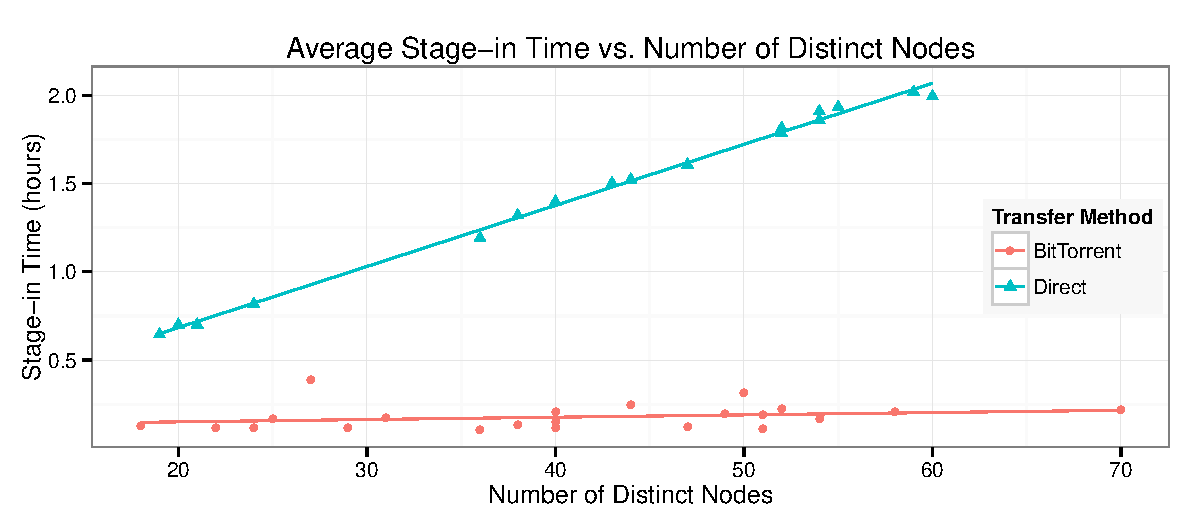
\includegraphics[width=\textwidth]{images/CombinedPlot.pdf}
\caption{Comparison of Direct and BitTorrent Transfer Methods with Increasing Distinct Node Counts}
\label{fig:combinedgraph}
\end{figure*}

Figure \ref{fig:combinedgraph} shows that the BitTorrent transfer method is superior to Direct for all experiments that were run.  Since multiple CacheDs on the same node will parent to a single CacheD, the number of distinct nodes is the dependent variable.  After the parent cache downloads the cache for the node, then each child cache will download from the parent using the Direct transfer method.

The Direct method of transfer follows a linearly increasing time to download the cache files.  This can be explained by bottlenecks of the transfers between the host machine and the execution nodes.  The increase in number of distinct nodes increases the stage-in time for any individual node.

The average download times for BitTorrent stage-ins are also shown in Figure \ref{fig:combinedgraph}.  The stage-in time does not significantly increase as the distinct nodes increases.  This meets our expectations.  We expect this trend to continue as the number of distinct nodes increases since BitTorrent can use peers to speed up download time.

\begin{figure}[ht!]
\centering
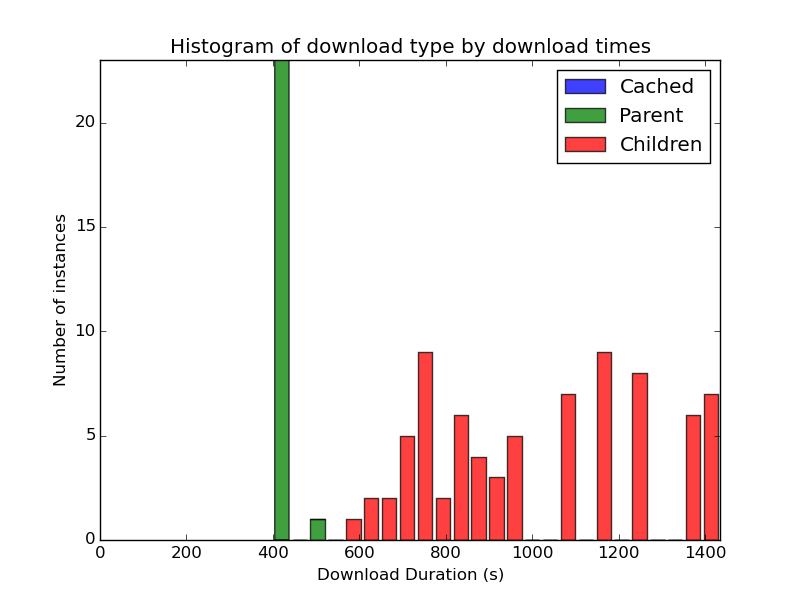
\includegraphics[width=0.5\textwidth]{images/modes_vs_downloadtimes.png}
\caption{Historgram of Transfers Mode vs Download Times}
\label{fig:histmethod}
\end{figure}

To better illustrate how parenting affects the download time of a cache, we show a histogram of the different modes in Figure \ref{fig:histmethod}.  The figure shows that while the parents download first, and nearly at all the same time, the children take a variable amount of time to download.  This variability can be attributed to the number of children on a node.  The more children downloading the cache at the same time, the slower each download will take. 

For our second experiment, we calculated the total stage-in time for a variable number of jobs.

\begin{figure*}[ht!]
\centering
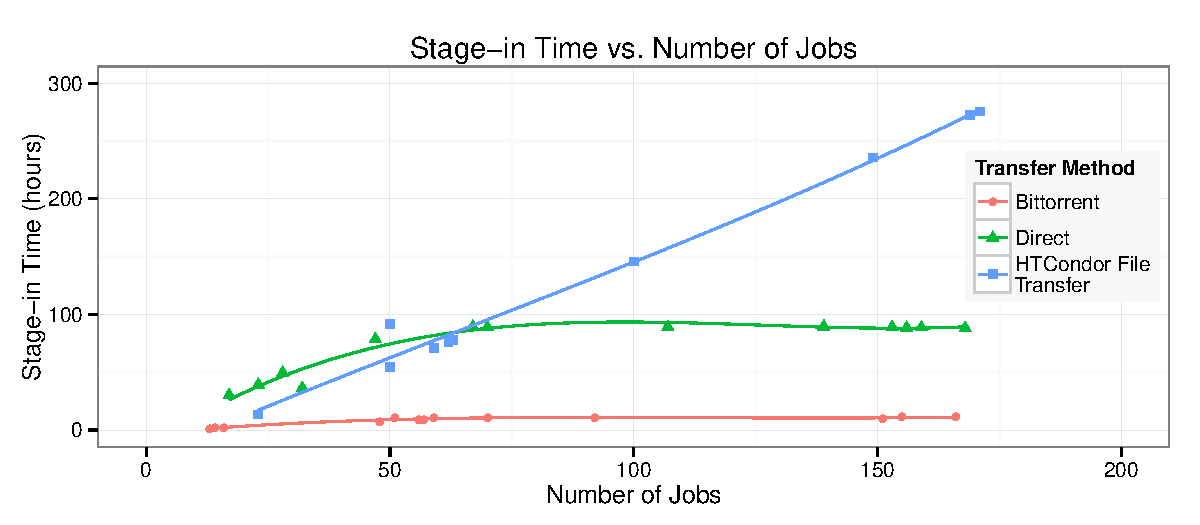
\includegraphics[width=\textwidth]{images/StageinPlot.pdf}
\caption{Transfer Method vs Number of Jobs}
\label{fig:methodvsnumjobs}
\end{figure*}

When we limit the number of nodes to 50, we can clearly see the effect of the caching by varying the number of jobs.  In Figure \ref{fig:methodvsnumjobs}, both the Direct and BitTorrent transfer methods have a natural bend at about 50 jobs.  This correlates to when the CacheD has on-disk caches of the datasets, and the transfer to the job's sandbox is nearly instantaneous.  

The HTCondor file transfer method has a shorter stage-in time for low numbers of distinct nodes than the Direct method.  This can be explained by the increased overhead that the CacheD introduces when transferring datasets.  After all 50 nodes have the dataset cached locally, the Direct transfer method becomes more efficient than the HTCondor file transfers.

%it begins with less overhead than the direct or the BitTorrent methods at low job counts.  But as the number of jobs increase, so to does the total stage-in time.  Since the condor file transfer method does not cache the data, it continues to linearly increase in stage-in time as the number of jobs increase.



\section{Conclusions}
We have presented the HTCondor CacheD, a technique to decrease the stage-in time for large shared input datasets.  Our experiments proved that the CacheD decreases stage-in time for these datasets.  Additionally, the transfer method that the CacheD used can significantly affect the stage-in time of the jobs.

The BitTorrent transfer method proved to be a efficient method to transfer caches from the originator to the execution hosts.  In fact, the transfer time for jobs did not increase as the number of distinct nodes requesting the data increased.  Any bottlenecks that surround the cluster are therefore irrelevant using the BitTorrent transfer method.

%For caching methods that attempt to optimize per cluster access, such as HTTP proxy methods, the results would like be very similar to those shown above.  Per cluster caching still bottlenecks the transfers to a single or set of nodes near the cluster.  They are better for optimizing latency of small accesses rather than aggregate bandwidth, which is required for large input datasets.

In the future we plan to investigate incorporating job matchmaking with cache placement.  The HTCondor Negotiator could attempt to match jobs first against resources that have the input files before matching against any available computing resources.


\section*{Acknowledgment}

This research was done using resources provided by the Open Science Grid, which is supported by the National Science Foundation and the U.S. Department of Energy's Office of Science.




